\begin{doublespacing}

\iffalse
A finite element model is created based on the TEM picture of irradiated U-10Mo. This particular research focuses on the distribution of Xenon bubbles inside the material and it impacts on thermal properties. The fission gas distributes itself in a regular pattern. It is called Gas bubble superlattice. The mechasim of formation of GBS is stilled needed to be understood. Eventhoug fission gas consits of Helium, Krypton and Xenon. Xenon percentage in the bubble is higher and also Xenon has the lowest thermal conductivity. Xenon percentage is also higher than krypton. For these reasons only Xenon's thermal conductivity is used in this research. A 2D geometry of two materials is created. One represents U-10Mo and other one is Xenon. The effective thermal conductivity of the unit cell is determined by applying a temperature difference across the boundary and solving for the temperature field within the geometry. In the current work MOOSE Framework is used to 
obtain the thermal solution.


A finite element model is used to represent a cross-sectional area(2D) of an intragranular space. The 2D mesh is created using Trimesh. Two material objects are created, one being U-10Mo and another one is Xenon. Thermal conductivity of U-10Mo is used from Burkes et. al~\cite{burkes2010thermo}. Different set of thermal conductivity of Xenon is used. The effective thermal conductivity of 
\fi

In this work, a Finite Element model is used to solve the steady state heat conduction equation to determinte the effective thermal conductivity of various fuel microstructures. Two types of microstructures were used as simulation domain. Both of the domains contain Xe bubble as fission product. One microstructure (Figure~\ref{fcc_mesh}) contains the Xenon Bubble superlattice sturcture and another microscturcture contains the grain boundary structure (Figure~\ref{fig_Xe_K}). The first one represents the intragranular bubble and the second one represents the intergranular bubble.
\begin{figure}
\centering
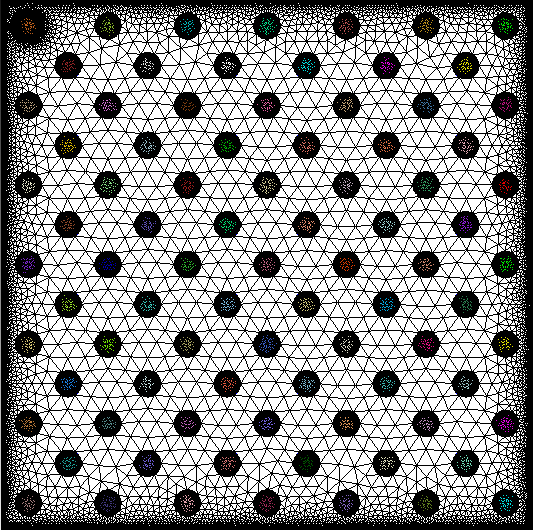
\includegraphics[scale=0.4]{figure_2D_fcc_r2_edited_white_BG.png}
\caption{Meshed Xenon bubble inside U-10Mo matrix}
\label{fcc_mesh}
\end{figure}
All simulations were performed in 2-D domain. The gas bubble supperlattice structure(GBS) was created based on Miller et al.~\cite{miller2015transmission}. According to Miller et al. the bubble size inside the GBS structure follows normal distribution. From these experimental values four diamters were chosen to create FEM model. Since, the GBS inside U-10Mo is FCC, the 2D sturcture was created based on the FCC sturcture. The lattice constant was 12 nm which was also from Miller et al. Lattice constants were kept constants for all four bubble sizes. The bubble sizes were 3.1, 3.6, 3.75 and 4 nm in diameter. The square domains dimension is $80\times80$ nm, with 91 bubbles inside it with lattice constants of 12. Two dimensional triangulare mesh was used to mesh the domain. Trelis Pro package was used to do the meshing. In the second microsturcture, grain boundary (GB) sturcture is created with Adobe illustrator. The size of the GB structure kept unchanged throughout the drawing. The GB sturcture of U-10Mo was chosen from Miller et al.~\cite{miller2012advantages}. This was a SEM (Scanning Electron Microscop image of a FIB (Focused Ion Beam) cross-section showing fission gas bubbles populating in the grain boundaries. This domain was also meshed with triangular mesh. A mesh study was done to chose a meshing size that will optimize the result and the compuational time. The effective thermal conductivity of the domain is determined by applying boundary conditions on each side  and solving for temperature field within the domain. In the current work MOOSE Framework~\cite{gaston2009moose} was used to obtain the thermal solution.

\begin{figure}[H]
\centering
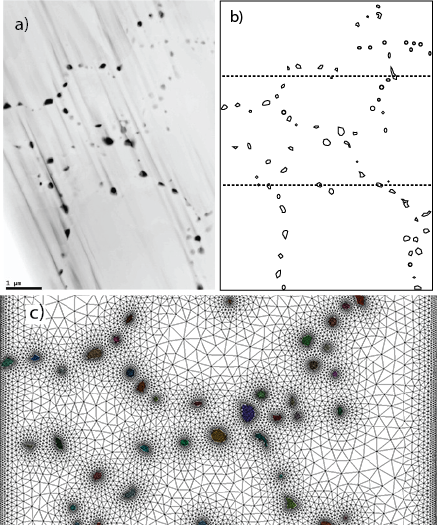
\includegraphics[scale=0.55]{grain_boundary_U-10Mo_white_BG.png}
\caption{a) TEM image of the fission gas bubbles along the grain boundaries from Miller et. al. used for FEM calculations~\cite{miller2012advantages} b) Geometry created based on the Grain Boundary fission gas modelling c)FEM mesh with grain boundary fissoin gas }
\label{fig_Xe_K}
\end{figure}



Two material objects were created. Both of these contained the thermal conductivity data for U-10Mo and Xenon. A linear fit of thermal conductivity with respect to temperature was used for U-10Mo which is from Burkes et. al.~\cite{burkes2010thermo}. Thermal conductivity of Xenon depends both on temperature and pressure~\cite{rabinovich1987thermophysical}. Figure~\ref{fig_Xe_K} shows the change of thermal conductivity with increasing pressure and temperature. Pressure inside the bubble highly depends on the radius and shear modulus of the host material~\cite{greenwood1959role,trinkaus1983energetics}. Xiao et. at.~\cite{xiao2015atomistic} performed atomistic simulation of the small Xenon bubble inside U-MO alloy. According to Xiau et. al. pressure inside the Xenon bubble can go as high as 12 GPa. This increased pressure creates another possibility of having solid Xenon bubbles inside the material~\cite{thomas1991condensed,ross1980condensed,zheng2014thermodynamics}. Thermal conductivity data of Xenon above 1000 bar is not available for a wide temeprature range. To evaluate the impact of pressure of Xenon on the overall thermal conductivity, five sets of thermal conductivity data (1bar, 70bar, 220bar, 380bar, 600bar and 1000bar) were used. For each set of data a polynomial fit is used for FEM calculation. The results are discussed in the following section.



\begin{figure}[H]
\centering
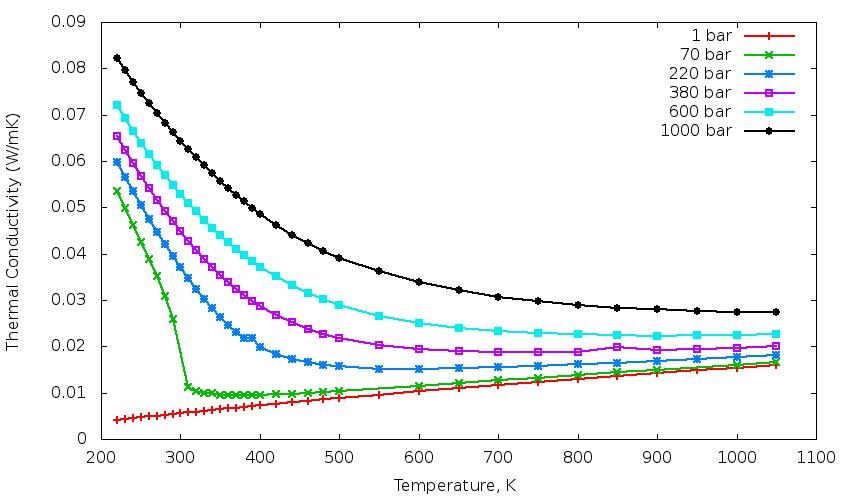
\includegraphics[scale=0.5]{Xe_K.png}
\caption{Thermal Conductivity of Xenon with increasing pressure from Rabinovich et. al.~\cite{rabinovich1987thermophysical}}
\label{fig_Xe_K}
\end{figure}



\end{doublespacing}
